% !TEX root = ../main.tex
\chapter{Introduction}
\label{chapter:Introduction}
Combination of quantum and classical computation as a form of heterogeneous computing allows us
to solve very interesting problems. Many quantum algorithms and applications relies
deeply on this combination. Whether near-time heterogeneous computing (i.e: Variational quantum eigensolver),
or real-time (i.e: quantum error correction algorithms). While near-time heterogeneous computing
is already achievable with current technology, albeit on a small scale, 
real-time heterogeneous computing is still a
challenge,
%TODO: fact check
due to the issue of decoherence time of quantum systems, and the requirement for
very low classical data transfer latency to account for this issue. In either
of these cases, we can use a quantum processing unit (QPU) as an accelerator
alongside a central processing unit (CPU), where the QPU can solve problems that QPUs excel in, and the
CPU can solve problems that CPUs excel in, such as conditionals, loops...etc.
This allows us to apply quantum algorithms that use a CPU as a coprocessor,
but also to improve the performance of a QPU as in the case of quantum error
correction.  This concept of heterogeneity can also be extended to include
other types of accelerators such as graphical processing units (GPUs), 
field programmable gate arrays (FPGAs), and application-specific integrated circuits (ASICs), to benefit from them
in domains where they excel. In this thesis we provide a compilation 
framework for OPENQASM 3.0, a quantum programming language that supports many classical instructions,
allowing for heterogeneous computing. Previous workflows have been provided towards this,
notably the QCOR framework \cite{qcor-openqasm}, which was a great inspiration for this work. QCOR, and after that this work,
created dialects for lowering of OPENQASM 3.0 to MLIR, apply optimizations and then
execute this intermediate representation on a QPU paired with a classical accelerator, or just execute it 
on a quantum simulator.
%maybe cite qcor?
In this work we approach this problem similarly, in a couple of aspects. Moreover, 
since the work on QCOR was discontinued, and the OPENQASM 3.0 spec was changing
frequently, and we wanted to keep up with the latest changes in the spec at the time of development.
% TODO: double check if we actually abide to the latest syntax,
% if not just mention that we tried to adhere to the latest available spec.
The differences in our approach are the following:
\begin{enumerate}
    \item Adhere to the latest spec as of time of development
    \item Use the latest MLIR version
    \item Make use of the latest MLIR dialects useful for our purposes. 
    \item Provide an explicit lowering step to a restricted quantum gates set, matching quantum gates
    available on desired hardware. We did this step as a proof of concept of the possibility to lower a generic quantum dialect
    to a restricted quantum dialect that has a specific set of quantum gates. We used quantum gates
    supported by the Walter Meiner Institute (WMI)'s quantum computers, as an example.
\end{enumerate}

In the next section we provide a background about the different topics relevant for this thesis. 
Followed by the body, where we showcase our approach to this
compilation pipeline, including the different steps involved in MLIR generation,
and finally we present some MLIR generated code and their corresponding stages in the compilation pipeline.

The different  MLIR generation step ranges 
from  showing the OPENQASM 3.0 code parse stage, to showing how we generate the corresponding
MLIR code in the quantum dialect -among other MLIR dialects- 
to applying optimizations - predefined classical ones and explicitly defined quantum optimizations,
to lowering this optimized MLIR code to have quantum gates only in the restricted quantum dialect,
to optionally generate a classical analog of all the quantum operations for our 
quantum operations to be simulated, and finally to lowering the MLIR code to LLVM IR for execution
by LLVM's Just-In-Time (JIT) compiler.
In the last section, we showcase a live-run of our quantum simulator along with its corresponding
quantum circuit, and provide some final closing remarks.

% This document has been created in order to show you some of the capabilities 
% of \LaTeX.  A great resource for an introduction to \LaTeX\xspace is Tobias
% Oetiker's ''The Not So Short Introduction to \LaTeXe'' \cite{latex}.  Please
% page through that document
% before starting with your thesis.
% Oh, and let's use the mysterious word \gls{computer} here to give the glossary
% a reason to appear.
% A third useful option to reference stuff besides citing or glossarying (?) 
% is using footnotes. Just like
% this\footnote{Properly formatted clickable URL: \url{https://www.tum.de/}}
% one.
% And: lists! Lists with bullet points are amazing. I mean, just look at this:
% \begin{itemize}
% 	\item list
% 	\item all 
% 	\item the 
% 	\item things!
% \end{itemize}
% % use enumerate for numbers instead of points: 
% % https://en.wikibooks.org/wiki/LaTeX/List_Structures#List_structures
% \par
% Anyways your introduction goes here.


% Below a few \LaTeX examples are included for beginners
% \comment{You can also put comments in the margins for you or your advisor}
% \begin{figure}[ht]
%   \centering
%   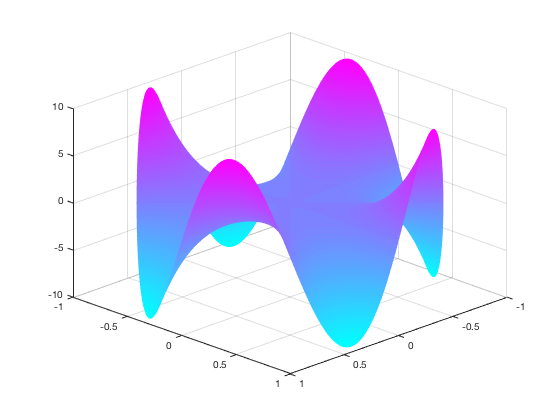
\includegraphics[width=5cm]{images/swing_function_plot.png}
%   \caption{$u(x)$}%{Numerically solved solution}
%   \label{fig:swingPlot}
% \end{figure}


% Equations can also be labeled
% \begin{equation}
% 	\pi = \mathrm{e}^{i\cdot\phi}
% 	\label{eq:equation1}
% \end{equation}


% And later referenced. Even in subfigures.
% \begin{figure}[!htb]
%   \centering
%   \begin{subfigure}[b]{0.3\textwidth}
%     \centering
%   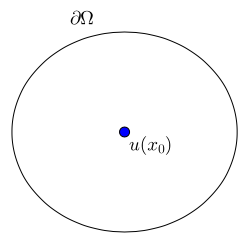
\includegraphics[width=\textwidth]{images/CircCenter}
%   \caption{Equation~\ref{eq:equation1}}\label{fig:circcenter}
% \end{subfigure}
% \hfill
%   \begin{subfigure}[b]{0.3\textwidth}
%     \centering
%   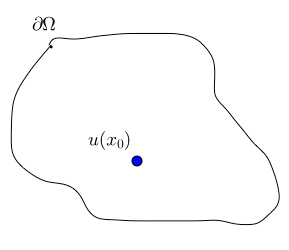
\includegraphics[width=\textwidth]{images/GeneralOffset}
%   \label{fig:generaloffset}
%   \caption{Equation~\ref{eq:equation1}}
% \end{subfigure}
% \end{figure}
% \section{Including code}

% Code can be using the package
% \href{https://www.sharelatex.com/learn/Code\_Highlighting\_with\_minted}{Minted}.

% An exaple of which of can be found below (see Source Code~\ref{lst:nice_listing})
% \begin{listing}
% 	%the language syntax can be declared here.
% 	\begin{minted}{python} 
% 	import numpy as np
	
% 	def incmatrix(genl1,genl2):
% 	    m = len(genl1)
% 	    n = len(genl2)
% 	    M = None #to become the incidence matrix
% 	    VT = np.zeros((n*m,1), int)  #dummy variable
	
% 	    #compute the bitwise xor matrix
% 	    M1 = bitxormatrix(genl1)
% 	    M2 = np.triu(bitxormatrix(genl2),1)
	
% 	    for i in range(m-1):
% 	        for j in range(i+1, m):
% 	            [r,c] = np.where(M2 == M1[i,j])
% 	            for k in range(len(r)):
% 	                VT[(i)*n + r[k]] = 1;
% 	                VT[(i)*n + c[k]] = 1;
% 	                VT[(j)*n + r[k]] = 1;
% 	                VT[(j)*n + c[k]] = 1;
	
% 	                if M is None:
% 	                    M = np.copy(VT)
% 	                else:
% 	                    M = np.concatenate((M, VT), 1)
	
% 	                VT = np.zeros((n*m,1), int)
	
% 	    return M
% 	\end{minted}

%   \caption{My nice listing}
%   \label{lst:nice_listing}
% \end{listing}
